\documentclass[12pt,preprint]{aastex}
\let\captionbox\relax
\usepackage{mathtools}
\usepackage{epstopdf}
\usepackage{amsmath}
\usepackage{graphicx}
\usepackage{caption,subcaption}
\usepackage{xcolor}
\usepackage{listings}
\captionsetup[figure]{labelsep=space,singlelinecheck=false}
\captionsetup[subfigure]{justification=centering}
% \epstopdfDeclareGraphicsRule{.pdf}{png}{.png}{convert #1 \OutputFile}
\graphicspath{ {images/} }
\DeclareGraphicsExtensions{.png,.pdf}

\begin{document}

% \title{Simulated CCD Exoplanet Photometry: High-Motion Space Telescopes}
\title{Simulated CCD Photometry: Low Pointing-Precision \textit{K2} Observations}

\author{Nicholas Saunders \altaffilmark{1,2}, Rodrigo Luger \altaffilmark{3,4}, Rory Barnes \altaffilmark{3,4}}

\altaffiltext{1}{NASA Ames Kepler/K2 Guest Observer Office, Mountain View, CA 94035}
\altaffiltext{2}{nicholas.k.saunders@nasa.gov}
\altaffiltext{3}{Department of Astronomy, University of Washington, Box 351580, Seattle, WA 98195, USA}
\altaffiltext{4}{Virtual Planetary Laboratory, Seattle, WA 98195, USA}

\begin{abstract}

	We present \texttt{scope} (Simulated CCD Observations for Photometric Experimentation), a \texttt{python} package to create a forward model of telescope detectors and simulate stellar targets with motion relative to the CCD. The primary application of this package is the simulation of the \textit{Kepler} Space Telescope detector to predict and characterize increased instrumental noise in the spacecraft's final campaigns of observation. As the fuel powering the spacecraft's stabilizing thrusters runs out and thruster fires begin to sputter or fail, stellar Point Spread Functions (PSFs) will experience more extreme and less predictable motion relative to regions of varied sensitivity on the spacecraft detector, generating more noise in transiting exoplanet light curves. Using our simulations, we demonstrate that current de-trending techniques  effectively capture and remove systematics caused by sensitivity variation for spacecraft motion as high as about ten times that currently experienced by \textit{K2}. The \texttt{scope} package is open-source has been generalized to allow custom detector and stellar target parameters. Future applications include simulating observations made by the Transiting Exoplanet Survey Satellite (\textit{TESS}), photometry and spectroscopy by the James Webb Space Telescope (\textit{JWST}), and ground based observations with synthetic atmospheric interference as testbeds for noise-removal techniques.

\end{abstract}

\section{Introduction}
\label{sec:intro}

Despite the failure of two reaction wheels in 2012 and 2013, the \textit{Kepler} Space Telescope has continued to produce valuable data in its new configuration, \textit{K2}, with significantly higher precision than ground based telescopes \citep{2014PASP..126..398H}. However, due to the unstable pointing caused by the missing reaction wheels, targets have significant motion relative to the quantum sensitivity variation of the telescope detector, creating noise in \textit{K2} light curves. A number of attempts have been made to isolate and remove the instrumental noise from \textit{K2} data \citep{2015A&A...579A..19A, 0004-637X-806-1-30, 2015MNRAS.454.4159H, 2015MNRAS.447.2880A, 2016MNRAS.459.2408A}. Through the appication of data processing pipelines, namely the \texttt{EVEREST} pipeline developed by \cite{2016AJ....152..100L}, the noise in \textit{K2} light curves can be reduced to the level of the original \textit{Kepler} mission for up to $15^{\text{th}}$ magnitude \citep{2017arXiv170205488L}.

However, as the \textit{Kepler} Space Telescope runs out of fuel, its motion due to thruster fires is expected to become less predictable and the magnitude of targets' motion relative to the detector will increase. With higher motion, targets will traverse more regions of varied pixel sensitivity, contributing more noise to the light curves of \textit{K2} targets. Eventually, when thruster fuel has been depleted entirely, the telescope may enter a phase of constant drift, at which point targets will traverse many pixels across the detector. This will also increase the likelihood of flux pollution from neighbors, as stellar PSFs may overlap over the course of a campaign.

In this paper, we present options for characterizing increased noise due to high motion and assessing noise-removal methods. \S 2 describes the mathematical methods of our simulation, \S 3 explores the results of our testing, \S 4 elaborates on future applications of this work, \S 5 provides usuage examples, and \S 6 discusses our conclusions.

\section{Methods}

Removal of instrumental noise requires a thorough understanding of its source. Stellar motion relative to the pixel sensitivity variation on the \textit{Kepler} CCD causes fluctuation in the amount of light received by the telescope detector over time. In order to accurately simulate the intrumental noise characteristic of \textit{K2} light curves, it is necessary to generate a forward model for the pixel sensitivity variation of the CCD. Light curves that were simulated using this sensitivity variation model are adequate to serve as well-understood sample targets on which to determine noise levels resulting from light curves generated under conditions of high roll magnitude and apply de-trending methods. To accurately represent the \textit{Kepler} CCD, we generated a model for the detector that included both inter-pixel sensitivity variation between pixels and intra-pixel sensitivity variation within each pixel.

\subsection{PSF Model}

A stellar PSF was generated with a characteristic two-dimensional Gaussian shape and with covariance between $x$ and $y$ dimensions to capture PSF distortion due to incident light aberration on the \textit{Kepler} detector. We define our model for $F(t)$, the total flux received by the telescope detector as a function of time, to be
%
\[
\tag{1}
F(t)=\sum_{aperture} \iint_{pixel} [s(x,y)P(x,y)\tau (t)]dxdy,\\
\]
%
where $s(x)s(y)$ is the sensitivity variation function, modeled by a sum of polynomials, and $P(x,y)$ is the PSF of the star, centered at $(x_0,y_0)$ with amplitude $A$. $\tau (t)$ is a simulated transit function. The pixel sensitivity model is given by the bivariate polynomial
%
\[
\tag{2}
s(x,y) = \sum_n a_{x,n}x^na_{y,n}y^n, \\
\]
%
and the PSF model is given by a sum over two-dimensional Gaussians
%
\[
\tag{3}
\begin{split}
P(x,y) & = \sum_m \frac{1}{2\pi\sigma_{x,m}\sigma_{x,n}\sqrt{1-\rho_m^2}} \text{exp}\left[ -\frac{1}{2(1-\rho_m^2)} \left( \frac{(x-x_{0,m})^2}{2\sigma_{x,m}^2} \right. \right. \\
			 & \phantom{xxxxx} \left. \left. + \frac{(y-y_{0,m})^2}{2\sigma_{y,m}^2} - \frac{2\rho_m  (x-x_{0,m})(y-y_{0,m})}{\sigma_{x,m}\sigma_{y,m}} \right) \right]
\end{split}
\]
%
where $\sigma_x$, $\sigma_y$ are the standard deviations of the PSF in $x$ and $y$, and $\rho$ is the correlation coefficient between $x$ and $y$.

This is the same model we fit to the simple aperture photometry (SAP) flux of \textit{K2} targets to subtract contaminant flux (further discussion in \S 4.1). The coefficients $a_n$ were determined to emulate the magnitude of sensitivity variation on the \textit{Kepler} CCD based on its contribution to the noise in \textit{K2} light curves. Sensitivity coefficients are defined as independent in $x$ and $y$ for consistancy with the Kepler Intrument Handbook \citep{kepler_intrument_handbook}. Our method for choosing values for sensitivity variation coefficients $a_n$ is descried in the following section.

\subsection{Pixel Sensitivity Variation}

Our model for the sensitivity variation was chosen to capture the same noise magnitude as real \textit{K2} targets. For our noise metric, we use the Combined Differential Photometric Precision for consistency with \cite{2016AJ....152..100L}. We used a two-step benchmarking process to estimate the magnitude of variation in quantum sensitivity and contribution by photon noise and background noise.

First we considered the no-motion case. For a large population of simulated targets with randomly generated stellar magnitude and detector position, the noise versus magnitude trend should closely follow that of the original \textit{Kepler} mission. The results of  Benchmark Test 1 are shown in Figure \ref{fig:nomotion}, where we plot the CDPP of our simulated light curves with no motion against CDPP of original \textit{Kepler} light curves as a function of \textit{Kepler} Magnitude ($Kp$ Mag).

To most accurately capture the characteristics of \textit{K2} data when analyzing the noise contributed by quantum sensitivity variation, our model included two sources of synthetic noise -- photon noise and background noise -- which contribute to the trend of increased noise for higher magnitude targets. Benchmark Test 1 serves to constrain the levels of injected photon noise and background noise. The test consisted of plotting the CDPP for 1,000 targets from the original \textit{Kepler} mission and calculating the median value for each $Kp$ Mag at intervals of 0.5. Next we generated five synthetic light curves for each 0.5-Mag interval, with the following random variation of parameters: centroid position of PSF varied by up to 0.2 pixels in both $x$ and $y$, $\sigma_x$ and $\sigma_y$ varied up to 10\% (${\sim}0.05$ pixels), correlation coefficient $\rho$ varied up to 40\%, and inter-pixel sensitivity varied up to 1\%. Each of these five simulated light curves is plotted against the \textit{Kepler} noise trend. This test was run iteratively on varied values of both background and photon noise until the slopes of the two trends approximately corresponded. To see the comparative noise of the resultant simulation, see Fig. \ref{fig:nomotion}.

\begin{figure}[h]
	\centering
	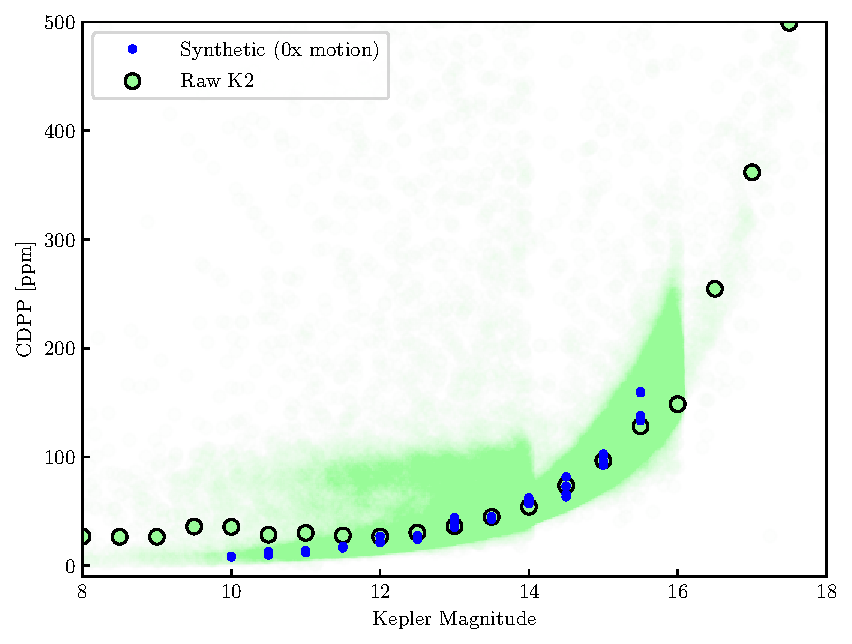
\includegraphics[width=1.0\linewidth]{kepler_benchmark.pdf}
	\caption{Benchmark Test 1: Noise level (CDPP) of our simulated light curves with no motion compared to original \textit{Kepler} targets as a function of $Kp$ Mag. The red trend demonstrates the relationship between $Kp$ Mag and noise for the \textit{Kepler} detector with high pointing precision, with the median represented by the larger red circles outlined in black. Each blue point is a simulated light curve with no motion vectors injected into the centroid position of the PSF. The primary contributors to this trend are photon noise and background noise, which were calibrated in our simulation by matching the slope of the \textit{Kepler} trend.}
	\label{fig:nomotion}
\end{figure}

In Benchmark Test 2, we consider the case of current \textit{K2} motion. To accomplish this, we injected motion from 1,000 cadences of the \textit{K2} target EPIC 205998445, creating a simulated example of a current observation to benchmark our model against \textit{K2} data. EPIC 205998445 is a \textit{K2} C03 star with $Kp = 12.029$ located ${\sim}60\%$ of the distance from the center of the detector plane to its edge. Statistics about the motion data used in our simulation can be found in Table \ref{table:motionstatistics}. This star was chosen because it is an isolated $12^{\text{th}}$ magnitude star, and the peak of the magnitude distribution for C03 was roughly 12. It is also located far enough from the center of the detector that it experiences significant motion during roll events, but not too near the edge that its motion is uncharacteristically high for \textit{K2} targets.

With real \textit{K2} motion applied, sensitivity variation parameters were adjusted until CDPP versus $Kp$ Mag correspended to the trend of real \textit{K2} observations. We found that a stochastic distribution of sensitivity with ${\sim}1\%$ variation between pixels and ${\sim}5\%$ variation within pixels, from center to edge resulted in Benchmark Test 2 following the expected trend most similarly. The results of Benchmark Test 2 can be seen in Figure \ref{fig:1motion}.

\begin{figure}[h]
	\centering
	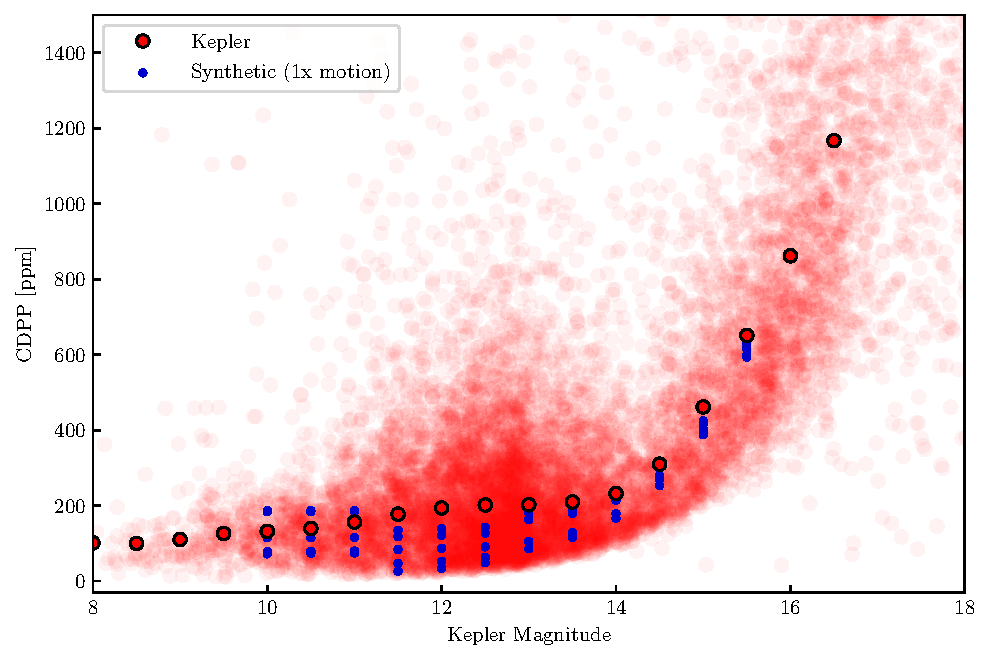
\includegraphics[width=1.0\linewidth]{k2_benchmark.pdf}
	\caption{Benchmark Test 2: Noise level (CDPP) of our simulated light curves with \textit{K2} motion compared to real \textit{K2} targets as a function of $Kp$ Mag. The points displayed in green show the noise of 1,000 raw \textit{K2} observations before de-trending with the EVEREST pipeline, and the larger green points outlined in black follow the median of the trend. Each blue point is a simulated target with current \textit{K2} motion and randomly varied initial centroid position and PSF shape. Our simulated data follow the same CDPP vs. $Kp$ Mag relationship as real data, indicating that the sensitivity variation in our model appropriately captures the detector.}
	\label{fig:1motion}
\end{figure}

A sample detector with included sensitivity variation can be seen in Figure \ref{fig:detector_sensitivity}. The calculation used in our simulation does not generate the sensitivity model and PSF individually, and instead passes the parameters into a singl -integrated function. This saves a computational step and speeds up the process. However, we were unable to solve the second integral prior to calculation because the first integral of a Gaussian results in an error function, which is non-analyitic.

\begin{figure}[h]
	\centering
	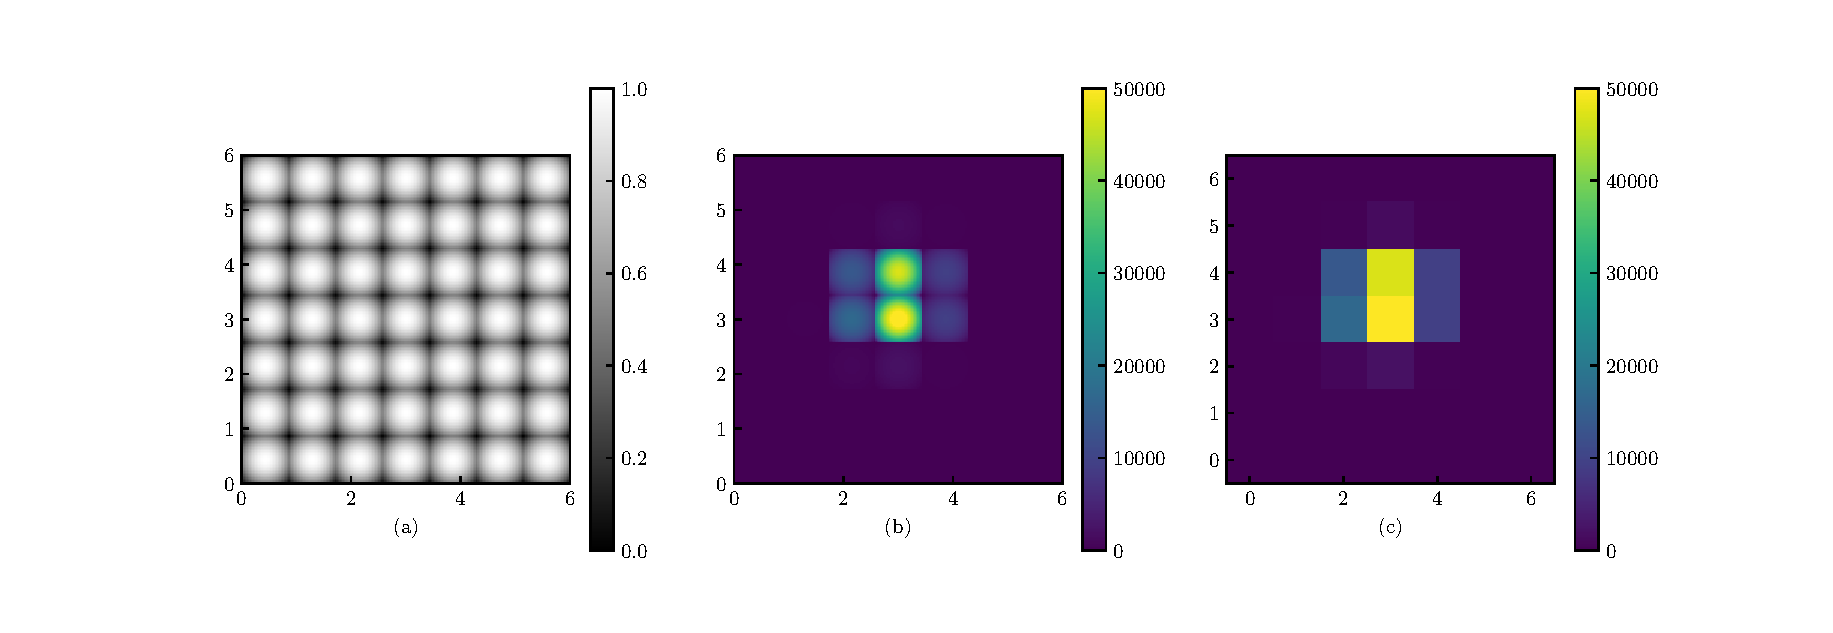
\includegraphics[width=1.0\linewidth]{detector_sensitivity.eps}
	\caption{(a) A sample detector with sensitivity variation and no stellar targets, where white represents 100\% photon detection efficiency, and the shaded regions have lower values for quantum sensitivity. Note that our model peaks in sensitivity at the center of each pixel and falls off towards the edges. There is also random variation in sensitivity between pixels. (b) A Stellar PSF mathematically simulated onto the detector at the sub-pixel level. The sensitivity variation has been exaggerated in this simulation to demonstrate the variation in sub-pixel fluxes. (c) The final interpolated image. The value of each pixel is the integral over $x$ and $y$ of the sub-pixel flux.}
	\label{fig:detector_sensitivity}
\end{figure}

For campaigns up to 17, stellar PSFs already traverse various regions of sensitivity variation on the CCD due to pointing instability. As spacecraft motion increases, PSFs will move more dramatically across many pixels, which will contribute significant noise to sputtering-\textit{K2} light curves.

\subsection{Increased Motion}

To test how PLD performs on targets with high motion relative to the detector, we injected motion vectors with various coefficients into our synthetic models. A coefficient of 1 corresponds to physical \textit{K2} motion (maximum of $\sim 0.59$ pixels), while a coefficient of 10 results in motion of up to $5.85$ pixels. More detail about motion can be found in Table \ref{table:motionstatistics}.

\begin{table}[h!]
\begin{center}
    \begin{tabular}{c | c | c | c | c}
        Coefficient & Motion (pix) & Max Motion (pix) & Motion (arcsec) & Max Motion (arcsec) \\
        \hline \hline
        1 & $0.17\pm0.12$ & 0.59 & $0.67\pm0.47$ & 2.33 \\
        2 & $0.34\pm0.24$ & 1.17 & $1.34\pm0.95$ & 4.66 \\
				5 & $0.84\pm0.59$ & 2.93 & $3.34\pm2.37$ & 11.65 \\
				10 & $1.68\pm1.19$ & 5.85 & $6.68\pm4.74$ & 23.30 \\
   \end{tabular}
	 \caption{Coefficients applied to the motion vectors of \textit{K2} target EPIC 205998445, an isolated C03 star. A coefficient of 1 corresponds to current motion, and each subsequent coefficient simply increases the motion by that factor. Motion is given in both pixels (pix) and arcseconds (arcsec).}
	 \label{table:motionstatistics}
\end{center}
\end{table}

Our method to increase motion involved simply multiplying the pixel offset due to current \textit{K2} motion by constant coefficients. This ensured the target traversed more pixels over a wider range of the detector while keeping the calculation simple enough to avoid introducing new opportunity for error. Because it is still unclear exactly how increased motion will manifest in the spacecraft's observations when fuel is expended, we opted to examine the simplest case. It should be noted that this may not be the most appropriate treatment for all de-trending methods, but because the method used in the \texttt{EVEREST} pipeline (pixel level decorrelation) is agnostic to cetroid position, our treatment of motion is thorough enough for the goal of testing noise-removal methods. \textcolor{red}{\textbf{Figure out how to say more about this.}}

\section{Results}

With a robust forward model of \textit{K2} established, including both motion and sensitivity variation, we were able to apply our de-trending methods to stars with various tiers of increased motion to predict and understand the results of thruster failure. To elaborate on the results of our test, we first discuss the details of our de-trending methods (\S 3.1), and then take a look at the application of these methods to our simulated data (\S 3.2).

\subsection{PLD}

After generating a set of light curves representative of extreme motion \textit{K2} observations, we tested systematics removal methods to assess how potentially valuable sputtering-\textit{K2} data would be. To de-trend our synthetic light curves, we used a variant of the method applied in the EPIC Variability Extraction and Removal for Exoplanet Science Targets (\texttt{EVEREST}) pipeline. The \texttt{EVEREST} pipeline utilizes a method called pixel level decorrelation (PLD), developed by \cite{0004-637X-805-2-132} for the \textit{Spitzer} Space Telescope.

PLD seeks to remove noise generated by intra-pixel sensitivity variation independent of apparent motion of the star. This method is particularly effective for \textit{K2} light curves despite the magnitude of apparent motion being high, and \texttt{EVEREST} can recover \textit{Kepler}-like accuracy in exoplanet light curves for targets up to $\text{Kp} = 15$. For a more detailed treatment of PLD, see the paper by \cite{0004-637X-805-2-132} and the first two \texttt{EVEREST} papers \citep{2016AJ....152..100L,2017arXiv170205488L}.

\subsection{Motion Tests}

When de-trended with second order PLD, our synthetic light curves align with the noise of original \textit{Kepler} observations for motion coefficients of 1x and 2x. 5x and 10x motion show increased noise in the de-trended light curve, but still perform better than observations from the ground. A detailed look at these results can be found in Figure \ref{fig:detmotion}.

\begin{figure}[h]
	\centering
	\includegraphics[width=1.0\linewidth]{detmotion.png}
	\caption{Noise level (CDPP) of simulated light curves after de-trending with $2^{\text{nd}}$ order Pixel Level Decorrelation (PLD) as a function of $Kp$ Mag. The green points show noise levels of 1,000 targets from the original \textit{Kepler} mission with the median represented by the larger green circles outlined in black. De-trended simulated light curves with 1x, 2x, 4x, and 10x current \textit{K2} motion are represented by the solid trends, and each point is the mean of 5 simulated light curves of a given $Kp$ Mag with slightly varied PSF shape and initial centroid positions. We achieve sub-400 ppm CDPP up to 5x motion for targets up to $Kp \text{ Mag}=15.5$, and de-trended light curves perform better that group based observation up to 10x motion.}
	\label{fig:detmotion}
\end{figure}

These results were achieved by applying second order PLD to pixels within an aperture around our simulated stars. The aperture is defined to exclude extraneous background and photon noise in order to maximize light from our target. In applications for real targets, it is often necessary to also consider nearby bright stars when defining an aperture. Future consideration will be given to automating aperture definitions, particularly because high motion PSFs will traverse more pixels and will therefore have a higher likelihood of crowding.

Our tests found that \texttt{EVEREST} and PLD are capable of removing instrumental noise from light curves of simulated targets with significantly increased magnitude of motion. The question surrounding the usefulness of high-motion data is very relevant to making decisions about the future of \textit{K2} observations, and our hope is to emphasize the potential value in continued observation and contribute to the de-trending of future data.

\section{Additional Discussion}

\textcolor{red}{\textbf{Condense into one section.}}

\subsection{Focus Changes}

Due to the internal optics of the Transiting Exoplanet Survey Satellite (\textit{TESS}), observed stellar PSFs may be large relative to the pixels on the CCD. Further, the space telescope's trajectory could cause a periodic variation in the incident sunlight on the telescope, which will affect the quantum sensitivity of pixels. Periodically changing sensitivity could cause \textit{TESS} PSFs to ``breathe" as the temperature rises and falls, and apertures around \textit{TESS} targets will need to expand and contract correspondingly to effectively capture the desired stellar signal. Our forward model serves as an established simulation for cases of time-variable PSFs due to both motion and periodic sensitivity changes.


\subsection{Increased \textit{TESS} Motion}

In the instance that \textit{TESS} also faces motion issues, there will be a significant need to test de-trending methods with an emphasis on defining ideal apertures. With a combination of large PSFs and increased noise, apertures and associated aperture-based PLD methods will be an essential piece of our noise-removal strategy for \textit{TESS}.

The stellar PSF parameters can be easily adjusted in the forward model produced by \texttt{scope} to cover more pixels and more accurately capture PSFs characteristic of \textit{TESS} observations. Using this simulation, it would be valuable to test various apertures and motion cases prior to the first public release of observations.

\subsection{Ground-based Observations}

Seeing aberation and atmospheric interference are additional sources of noise that could be included in the \texttt{scope} model. PLD was developed for \textit{Spitzer} and modified for application to \textit{K2}, but has seen little application elsewhere. For ground-based observations with significant noise due to pointing issues or atmospheric interference, PLD may be a valuable tool to make the most of data. \texttt{scope} is an ideal testbed for this type of noise-removal because it allows users to perform tests on noisy observations performed on sources that are well understood with input parameters that can be compared to post-processing results. Though it was initially imagined for space-based telescopes, this software has potentially useful applications for ground-based telescopes.

\section{Using \texttt{scope}}

All of our code is open-source and publically available online. Our simulation package can be installed by running
%
\begin{lstlisting}[language=bash]
pip install tele-scope
\end{lstlisting}
%
To create a light curve with \texttt{scope}, first instantiate a \texttt{Target} object:
%
\begin{lstlisting}[language=Python]
import scope
star = scope.Target()
\end{lstlisting}
%
A light curve can be generated by calling the \texttt{GenerateLightCurve()} function, which returns a light curve of target pixel files (\texttt{fpix}), a one-dimensional flux light curve (\texttt{flux}), and a light curve of the error in each pixel (\texttt{ferr}):
%
\begin{lstlisting}[language=Python]
fpix, flux, ferr = star.GenerateLightCurve()
\end{lstlisting}
%
After a target is created, transits, variability, or neighbors can be added with the following functions:
%
\begin{lstlisting}[language=Python]
star.AddTransit()
star.AddVariability()
star.AddNeighbor()
\end{lstlisting}
Alternatively, the target can be initialized with added features by changing the following boolean parameters:
%
\begin{lstlisting}[language=Python]
star = scope.Target(transit=True, variable=True, neighbor=True)
\end{lstlisting}
%
The detector with sensitivity variation can be displayed by calling
%
\begin{lstlisting}[language=Python]
star.DisplayDetector()
\end{lstlisting}
%
To de-trend with second order PLD, run
\begin{lstlisting}[language=Python]
star.Detrend()
\end{lstlisting}
\section{Conclusions}

We have created a forward model of the \textit{Kepler} space telescope detector, \texttt{scope}, which includes inter- and intra-pixel sensitivity variation and mathematical simulations of stellar PSFs to test de-trending methods for exoplanet targets. Using these simulations, we have demonstrated that \texttt{EVEREST} and PLD are  capable of reducing systematic noise to higher precision than ground based observations in \textit{K2} light curves with up to 10x current spacecraft motion. We have shown that in the event of spacecraft thruster sputtering due to diminishing fuel reserves, valuable data can still be collected and analyzed to benefit \textit{K2} science goals.

Though \textit{TESS}, the successor to \textit{Kepler}, has launched, there remains a wealth of both existing and unobserved \textit{K2} data that offers valuable contribution to our understanding of exoplanetary systems. Earthlike exoplanets can be difficult to identify in the high-magnitude noise of current \textit{K2} data, which will continue to get noisier as the mission reaches its conclusion. The methods we have presented aim to produce the most precise exoplanet identification, characterization, and analysis from the data we have available, and prepare for the next generation of space telescopes.

This work was supported by NASA grant NNX14AK26G and by the NASA Astrobiology Institute's Virtual Planetary Laboratory. Computing for this research was performed on the Hyak supercomputer system at the University of Washington.

\clearpage
\bibliographystyle{aasjournal}
\bibliography{references.bib}

\end{document}
